\documentclass[12pt,tikz]{standalone}
% \documentclass[12pt,a4paper]{standalone}
% \documentclass[tikz,a4paper]{standalone}

\usepackage{tikz,rotating}
% \usepackage{tikz,rotating,fullpage,anysize}
\usetikzlibrary{decorations.pathmorphing,decorations.text}

\pagestyle{empty}
% \marginsize{1em}{1em}{1em}{1em}
% \cleardoublepage
% \clearpage
\standaloneconfig{border=2em}

\Large

\begin{document}


\pgfdeclarelayer{background}
\pgfdeclarelayer{main}
\pgfsetlayers{background,main}

\begin{tikzpicture}
\centering
  % \draw [help lines] grid (10,18);
    % {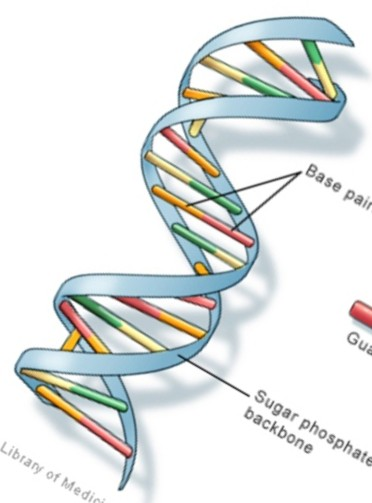
\includegraphics[width=\paperwidth,height=\paperheight]{dna.jpeg}};
  % \begin{pgfonlayer}{background}
  %     % {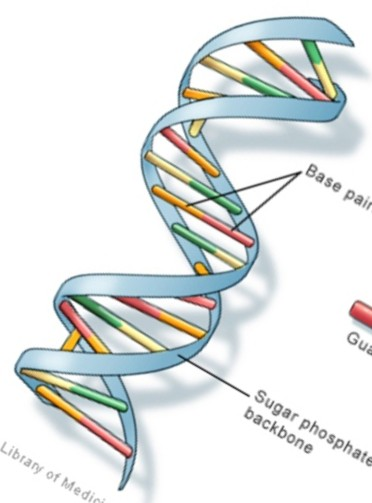
\includegraphics[height=\textheight,keepaspectratio]{dna.jpeg}}
  %     {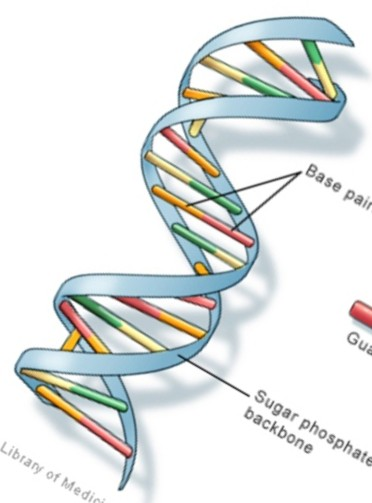
\includegraphics[height=29cm,keepaspectratio]{dna.jpeg}}
  % \end{pgfonlayer}
  % \draw[gray,line width=1pt] (current page.south east) rectangle (current page.north west);
  \begin{pgfonlayer}{main}
    % grid
    % \draw [step=1.0,gray,thin] (0,0) grid (21,29);

    % help line
    % \draw  (2,0) -- (18,29);

    % draw top text on curvy path
    \path [decorate,decoration={text along path,
            text align = fit to path,
            text={|\Large|When ivy trails along the ground it remains weak and does not\space\space\space\space\space\space\space\space\space\space\space produce fruit, but when it climbs a tree or\space\space\space\space\space \space\space a wall for support it grows increasingly stronger. *}}]
      (3,6) -- (1.5,8)  
      .. controls (2,9) and (9.3,6.5) .. (12.2,9.8)
      .. controls (14,12.5) and (6.5,20) .. (9,21.3)
      .. controls (10.8,23.8) and (19,21.5) .. (19.5,22.8)
      .. controls (20,24) .. (17,25.5);
    % draw bottom text on curvy path
    \path [decorate,decoration={text along path,
            text align = fit to path,
            % text width={\pgfdecoratedpathlength},
            text={|\Large|* Its botanical name is Hedera\space\space\space\space\space\space\space\space Helix and describes ivy's spiral form of growth, for helix means to turn around. The rich deep evergreen colour and climbing spiral action inspired +}}]
      (7,1)  
      .. controls (10,5.5) and (2.5,11.5) .. (3.5,12)
      .. controls (5,13.5) and (13,10.8) .. (14.5,13.8)
      .. controls (15.5,16) and (9,23) .. (11,25)
      .. controls (11.8,26.5) and (15.5,27.5) .. (19.5,27);

    \path (15,25) node [rotate=-25, node font=\Large] {+ the ancients}
          (14,24.2) node [rotate=-25, node font=\Large] {to identify}

          (10.2,20.3) node [rotate=-20, node font=\Large] {ivy with}
          (10.8,18.7) node [rotate=-20, node font=\Large] {resurrection}
          (12,17.2) node [rotate=-20, node font=\Large] {and rebirth.}
          (12.2,16) node [rotate=-20, node font=\Large] {It was thought}

          (9,10.7) node [rotate=-20, node font=\Large] {that one spiral}
          (7.5,10.3) node [rotate=-20, node font=\Large] {reversed}
          (6,10) node [rotate=-20, node font=\Large] {the power}

          (5,6) node [rotate=-20, node font=\Large] {of the other.}
          ;

  \end{pgfonlayer}
\end{tikzpicture}


\end{document}